\documentclass[main.tex]{subfiles}

\begin{document}
	
\section{Pathophysiology}
	
\begin{figure*}[H]
	\centering
	\caption{Metabolism of Methemoglobin}
	\label{img:methgb-Metabolism}
	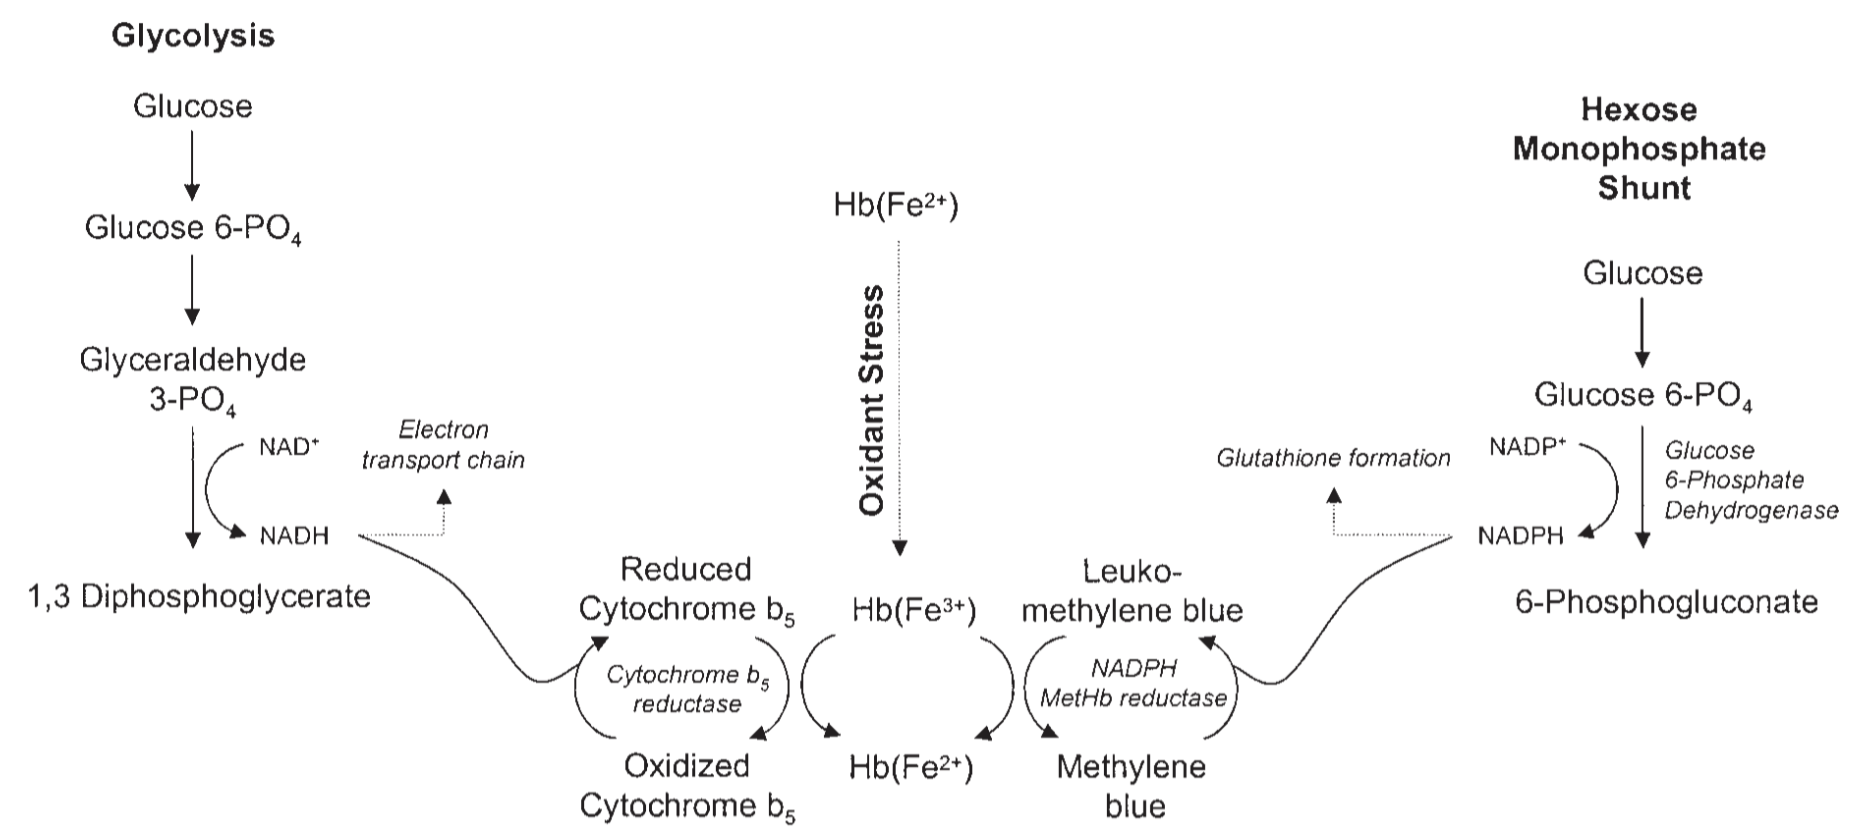
\includegraphics[width=\linewidth]{img/methemoglobinemia/metabolism.png}
	\raggedleft \footnotesize \textit{From Goldfrank's Toxicology (2007)}
\end{figure*}

\begin{itemize}[noitemsep]
	\item Oxidant stress converts hemoglobin iron from \ce{Fe^2+} to \ce{Fe^3+}
	\begin{itemize}[noitemsep]
		\item Still binds oxygen, but doesn't release it (shifts binding curve left)
	\end{itemize}
	\item NADH (glycolosis) pathway detoxifies most methemoglobin (Met-Hgb) during normal situations
	\item NADPH is upregulated when needed, such as toxin-induced methemoglobinemia
\end{itemize}

\begin{figure}[hbt]
	\centering
	\caption{Met-Hgb (left), Normal (right)}
	\label{img:methgb-picture}
	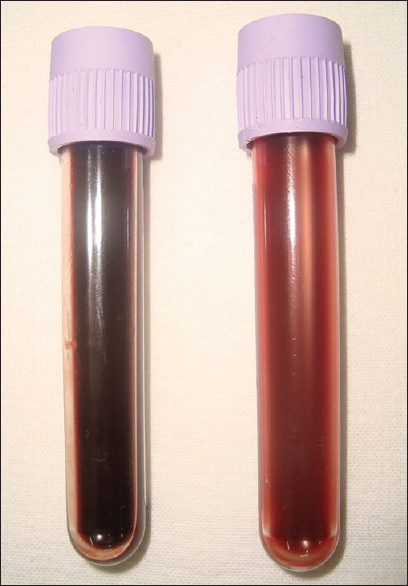
\includegraphics[width=0.6\linewidth]{img/methemoglobinemia/blood.jpg}\\
	\footnotesize DOI: \href{http://www.e-ijd.org/article.asp?issn=0019-5154;year=2015;volume=60;issue=1;spage=108;epage=108;aulast=Das}{10.4103/0019-5154.147895}
\end{figure}

\subsection{Causes}
	\begin{itemize}[noitemsep]
		\item Conditions
		\begin{itemize}[noitemsep]
			\item Cytochrome \ce{b_5} reductase deficiency
			\item Hemoglobin M
		\end{itemize}
		\item Drugs
		\begin{itemize}[noitemsep]
			\item \textbf{Dapsone}
			\item \textbf{Benzocaine} (and other local anesthetics)
			\item Nitrite-containing compounds (NTG, nitroprusside, amyl nitrite)
			\item Sulfonamides (sulfa antibiotics)
			\item Analine dyes
			\item Primaquine / chloroquine
			\item Many others
		\end{itemize}
	\end{itemize}

\begin{figure*}[hbt]
	\centering
	\caption{\textbf{Methemoglobin \%}}
	\label{img:methgb-gradient}
	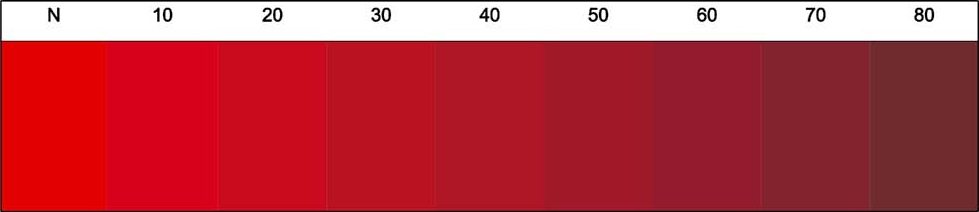
\includegraphics[width=0.8\textwidth]{img/methemoglobinemia/color-chart.png}\\
	\raggedleft \footnotesize Shihana et al. \hspace{0.1\textwidth}
	\caption*{\footnotesize \textit{Place a drop of blood on white paper, allow it to dry, and compare with chart above. Chart Met-Hgb should be within $\pm$ 15\% of lab value}}
\end{figure*}

\section{Diagnosis}

\begin{itemize}[noitemsep]
	\item \textbf{Be suspicious for methemoglobinemia in cyanotic patients with an SpO2 in the mid-80\%'s which is unresponsive to supplemental oxygen, and in patients with chocolate-colored blood}
	
	\item Hypoxic cyanosis usually doesn't occur until SpO2 is $\approx$50\%, this is a rare case of cyanosis with ``high" SpO2
	
	\item \textbf{SaO2 - SpO2 \textgreater 5\%} is an indication that something is messing with pulse-ox reading, usually a deviant Hgb like Met-Hgb
	\begin{itemize}[noitemsep]
		\item High Met-Hgb will make SpO2 trend toward $\approx$ 85\%
		\item Supplemental O2 will drive up PaO2, and SaO2 on iStat ABGs will increase because it is calculated from PaO2
	\end{itemize}
	
	\item Order methemoglobin from lab for confirmation, if symptomatic with high suspicion for methemoglobinemia, can treat empirically
\end{itemize}

\begin{table}[htb]
	\centering
	\rowcolors{2}{white}{tableColor}
	\caption{Met-Hgb Symptoms}
	\label{tab:methbg-SSx-percent}
	\begin{tabular}{ll}
		\textbf{Met-Hgb \%} & \textbf{Symptoms} \\ \hline
		1-3\% & Normal \\
		10-20\% & Cyanosis \\
		20-30\% & \begin{tabular}[c]{@{}l@{}}Anxiety\\ Headache\\ Dizziness\\ Fatigue\end{tabular} \\
		30-50\% & \begin{tabular}[c]{@{}l@{}}Tachypnea\\ Confusion\\ Syncope\end{tabular} \\
		50-70\% & \begin{tabular}[c]{@{}l@{}}Szs\\ Coma\\ Metabolic Acidosis\end{tabular} \\
		\textgreater{}70\% & Death
	\end{tabular}
\end{table}

\section{Treatment}
\begin{itemize}[noitemsep]
	\item \textbf{Treat symptomatic patients or any patient with Met-Hgb \textgreater 30\%}
	\item Call Toxicology
	\item Methylene Blue 1-2 mg/kg IV over 5 min
	\begin{itemize}[noitemsep]
		\item Can repeat in 30-60min if needed
		\item SpO2 may decrease significantly during infusion, caused by interference with pulse-ox, not hypoxia
		\item Will discolor body fluids
		\item Side effects
		\begin{itemize}[noitemsep]
			\item MAO inhibition $\implies$ serotonin syndrome
			\item Methemoglobinemia (doses \textgreater 7 mg/kg/day) 
		\end{itemize}
		\item May not be as effective for analine dye overdoses, analine metabolite inhibits entry of methylene blue into RBCs
	\end{itemize}
	
	\item Methylene Blue continuous infusion
	\begin{itemize}[noitemsep]
		\item Limited evidence for dosing
		\begin{itemize}[noitemsep]
			\item One case series reported 2 mg/kg over 6hr (0.33 mg/kg/hr, daily dose 8 mg/kg) 
			\item Some self-reporting from toxicologist starting at 0.1 mg/kg/hr
			\item Rates of 0.5-1 mg/kg/hr when used for vasoplegia, so higher doses \textit{may} be safe
			\item \textbf{Bottom line: Call tox if you have to start continuous methylene blue}
		\end{itemize}
		\item Usually not needed, consider if Met-Hgb induced by long-acting agent like dapsone, or if \textgreater 2 bolus doses needed
	\end{itemize}
	
	\item Cimetidine for Dapsone induced Met-Hgb
	\begin{itemize}[noitemsep]
		\item Inhibits CYP450 metabolism of dapsone $\to$ hydroylamine dapsone, which produces more Met-Hgb than dapsone
	\end{itemize}
	
	\item Other Therapies
	\begin{itemize}[noitemsep]
		\item High-Dose Vitamin C (takes a long time to work)
		\item Riboflavin (takes a long time to work)
		\item Hyperbaric oxygen
		\item Red-cell exchange
	\end{itemize}
\end{itemize}

\nocite{goldfrankGoldfrankManualToxicologic2007,ludlowMethemoglobinemia2019,prasadDapsoneInducedMethemoglobinemia2008,shihanaSimpleQuantitativeBedside2010,skoldMethemoglobinemiaPathogenesisDiagnosis2011}

\printmybib
	
\end{document}